\subsection{Einzelfunde}\label{sec:SHG-LKW_Einzelfunde}

Die Prospektion des \textit{River Reconnaissance Project} im Jahr 1985 entlang des \mbox{Ubangi} erbrachte neben den skizzierten keramischen Stilgruppen (Kap.~\ref{sec:BTM-Gr}--\ref{sec:BAN-Gr}) auch eine Reihe nicht zuordenbarer Einzelfunde. Dazu zählen vier hohe, spitzbodige Flaschen (Typ A1), die an drei Fundstellen am unteren \mbox{Ubangi} gefunden wurden (Abb.~\ref{fig:spitzbodigeFlaschen_Verbreitung}).\footnote{Zwei GE stammen aus Bolumbu (Fpl.~194, Taf.~4.8), während je eine GE in Bokwango (Fpl.~190; Taf.~2.2) und Loka (Fpl.~193) gefunden wurde.} \textcite[211--212]{Wotzka.1995} interpretiert entsprechende Stücke als Importe aus dem \mbox{Ubangi}- und Ngiri-Gebiet. Während sich entsprechende GE vereinzelt, allerdings ohne irgendeinen weiterführenden Kontext an den genannten Fundstellen am unteren \mbox{Ubangi} fanden, geht die Angabe Wotzkas, dass solche Gefäße vom zwischen dem Kongo und \mbox{Ubangi} verlaufenden Ngiri stammen können, auf eine Befragung Manfred Eggerts in Lokekya (Fpl.~188) zurück. Von der lokalen Bevölkerung wurde die Herkunft der Gefäße mit der angeblich noch 1985 in Bomongo am Ngiri (Abb.~\ref{fig:spitzbodigeFlaschen_Verbreitung}) betriebenen Töpferei in Zusammenhang gebracht (ebd. 211 Anm.~7). Eine unabhängige Verifizierung dieser Aussage, so zum Beispiel durch eine Befahrung des Ngiri und der damit verbundenen Beobachtung vor Ort, war damals nicht möglich. Entfernt ähnliche spitzbodige, hohe Flaschenformen sind auch aus dem Aruwimi-Gebiet bekannt \parencite[Taf.~XVII]{Coart.1907}.

\begin{figure*}[p]
	\centering
	\includegraphics[width=\textwidth]{fig/spitzbodigeFlaschen_Verbreitung.pdf}
	\caption{Einzelfunde: Verbreitung spitzbodiger Flaschen (Typ A1) im Arbeitsgebiet (Fpl.~188--194), dem Inneren Kongobecken \parencite[211f.; Fpl.~139--145]{Wotzka.1995} sowie ihr mutmaßlicher Herstellungsort Bomongo am Ngiri ({\footnotesize $\bigstar$}).}
	\label{fig:spitzbodigeFlaschen_Verbreitung}
\end{figure*}

Die genannten Flaschen zeichnen sich einerseits durch eine teilweise sehr hohe, schmale Grundform aus, mit Proportionen von Mündungshöhe zu maximalem Durchmesser von fast 3:1 bis 4:1 \parencites[siehe Taf.~4.8;][531 Taf. 97.10]{Wotzka.1995}[167 Abb.~III.11.1]{OmasomboTshonda.2014}, es sind jedoch auch deutlich stärker gebauchte Formen bekannt (Taf. 2.2). Der Großteil des Gefäßkörpers dieser Flaschen ist mit einem sehr tief eingearbeiteten \textit{banfwa-nfwa} (Tab.~\ref{tab:Verzierungselemente}: 08) verziert. Vergleichare in \textit{banfwa-nfwa}-Technik erzeugte Muster finden sich ausschließlich in jenen Stilen, die mit der jüngeren Phase der Keramiksequenz in Zusammenhang stehen \parencite[siehe Kap.~\ref{sec:BKW-Gr}, \ref{sec:EBA-Gr},][109--111]{Wotzka.1995}. Daher kann für die spitzbodigen Flaschen gegenwärtig nur von einem grundsätzlich jüngeren Alter ausgegangen werden. Auch die Berichte, dass sie noch 1985 in Bomongo am Ngiri gefertigt worden sein sollen, weisen auf ein rezentes, bis höchstes subrezentes Alter hin. Zusätzlich zu diesen archäologischen Funden befindet sich eine entsprechende Flasche im \textit{Musée royal de l'Afrique centrale} in Tervuren  \parencite[167 Abb.~III.11.1]{OmasomboTshonda.2014}.\footnote{Genauere Angaben, wann und wo die Stücke gesammelt wurden, sind nicht bekannt (\textsc{Omasombo Tshonda} 2014: 167 Anm.~83). Auf der Fotografie ist ebenfalls eine Schale mit Bauchknick vom Typ F3 zu sehen (ebd. 167 Abb.~III.11.1), die der Mobaka-Gruppe zugerechnet werden kann (Kap.~\ref{sec:MKA-Gr}). Diese Keramik kommt ausschließlich am unteren \mbox{Sangha} und dem \mbox{Likwala}-\mbox{aux}-\mbox{Herbes} vor (Abb.~\ref{fig:MKA_Verbreitung}). Die darüber hinaus abgebildeten Gefäße 1, 3 und 5 sind im hier analysierten Material nicht repräsentiert.}

\begin{figure*}[p]
	\centering
	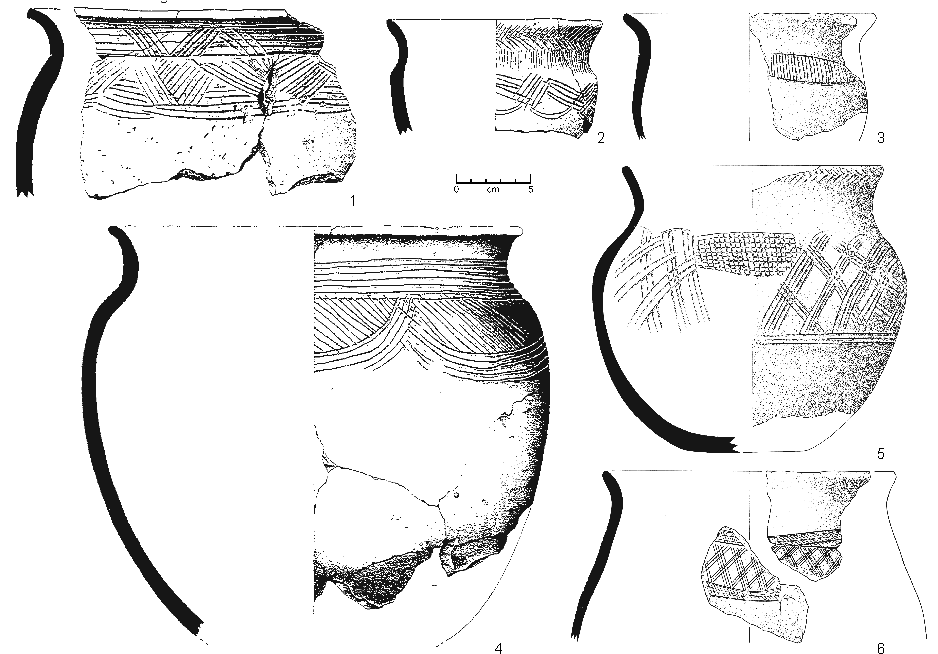
\includegraphics[width=\textwidth]{fig/Ngovo-Typen.pdf}
	\caption{Likwala-aux-Herbes, Flusskilometer 186: Typvertreter des Inventars der Grube LKW~87/186, Kat.-Nr.~19 (3, 5--6) sowie Vertreter der Ngovo-Gruppe des Niederkongos (1--2, 4).\\1:~\textcite[108~Abb.~4.7]{deMaret.1986}; 2:~(ebd. 108~Abb.~4.14); 3:~Taf.~76.2; 4:~(ebd. 111~Abb.~5.3); 5:~Taf.~76.1; 6:~Taf.~76.3.}
	\label{fig:Ngovo_Typvertreter}
\end{figure*}

Die Befahrungen des \mbox{Sangha}, \mbox{Ngoko} sowie Likwala-aux-Herbres im Jahr 1987 erbrachten neben den beschriebenen Stilgruppen (Kap.~\ref{sec:PKM-Gr}--\ref{sec:BBS-Gr}) weitere keramische Phänomene, die als isolierte Einzelfunde keine dedizierten Aussagen zum Besiedlungsgang des Arbeitsgebietes erlauben.

\begin{figure*}[p]
	\centering
	\begin{minipage}[b]{\columnwidth}
		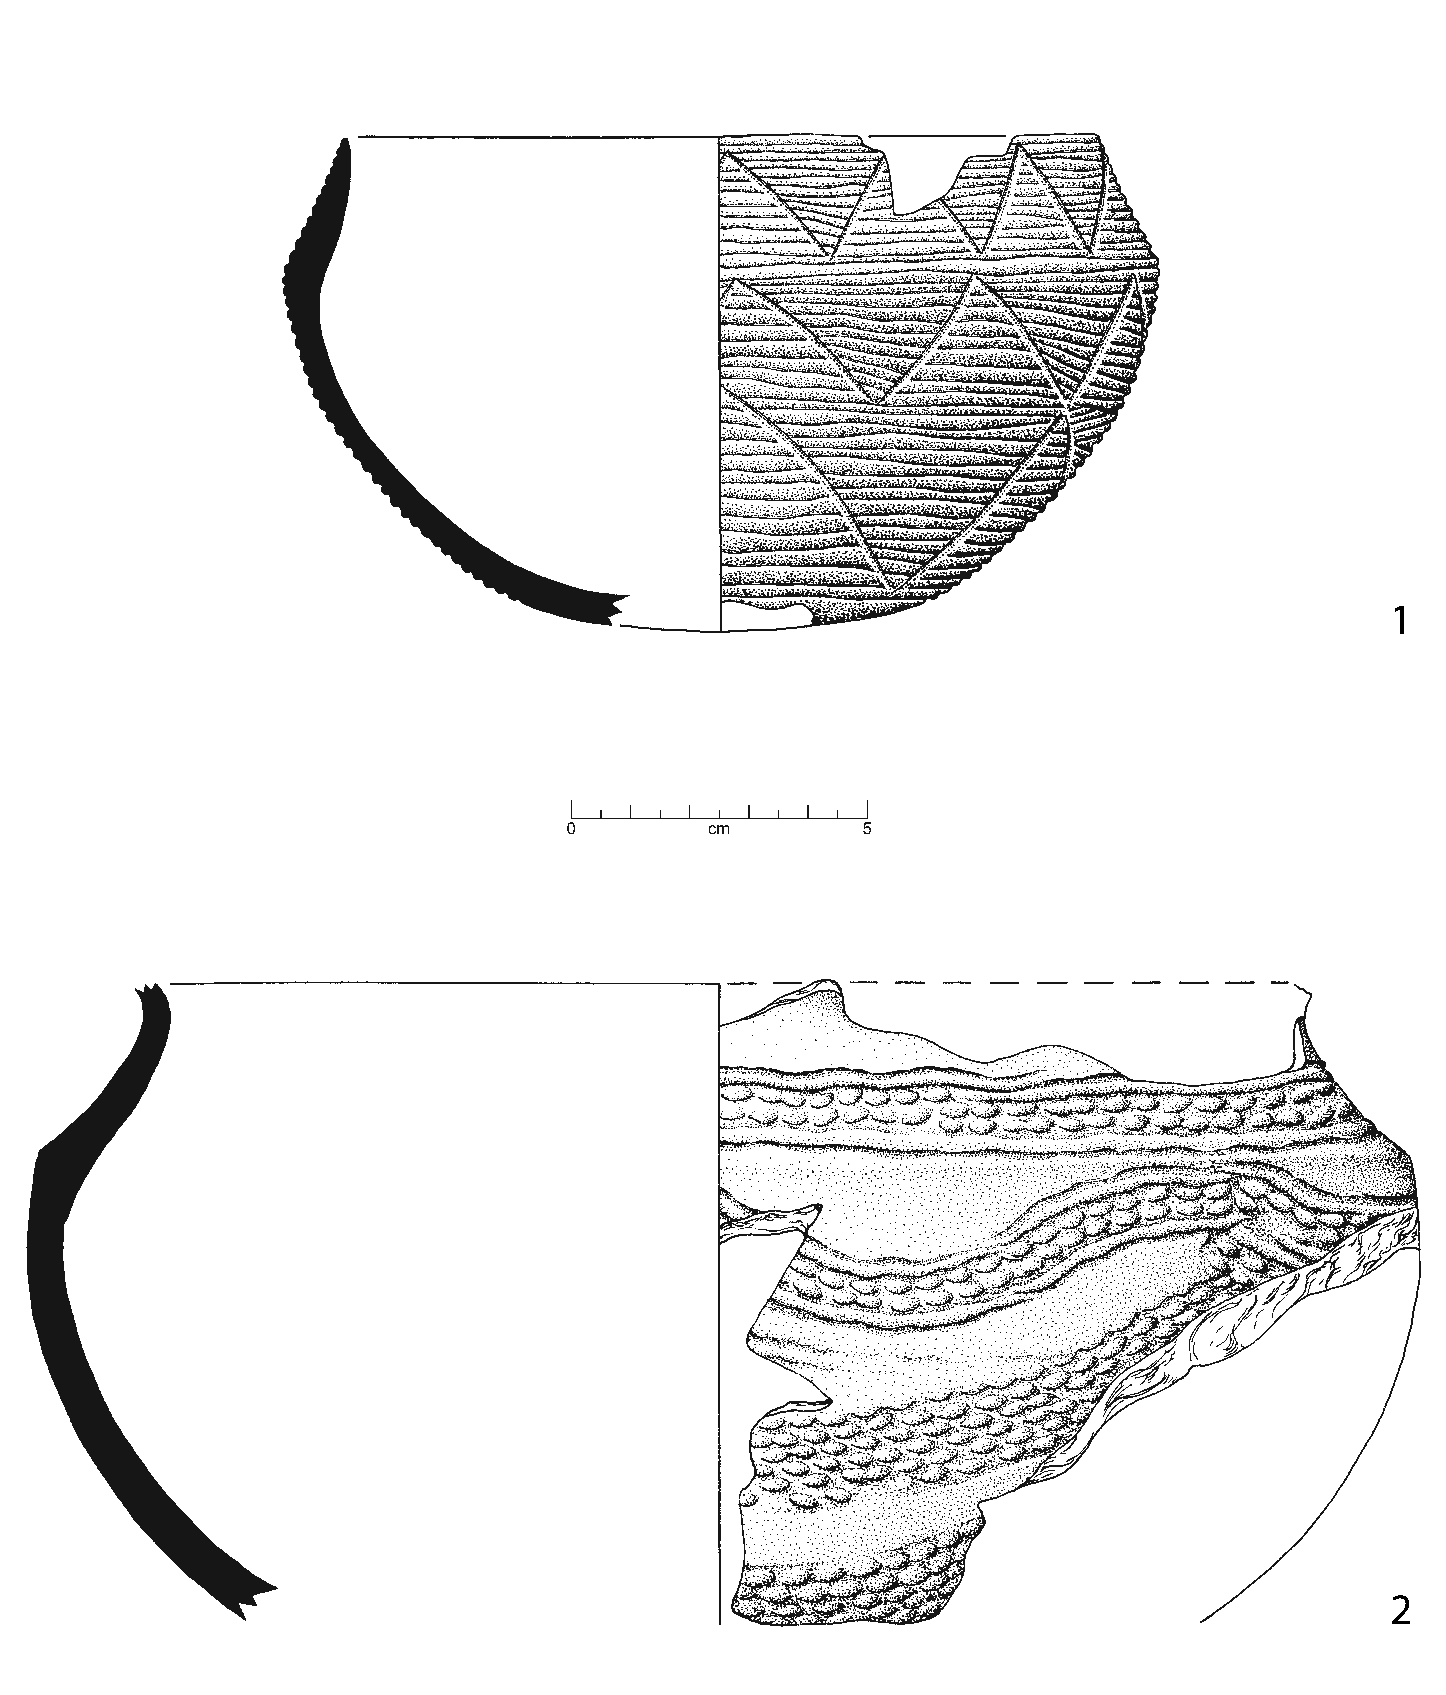
\includegraphics[width=\textwidth]{fig/MPB87-101_Typen.pdf}
		\caption{Mai~mpembe (Fpl.~271).\\1:~Taf.~62.5; 2:~Taf.~62.4.}
		\label{fig:MPB87-101}
	\end{minipage}\hfill
	\begin{minipage}[b]{\columnwidth}
		\includegraphics[width=\textwidth]{fig/SSL87-101_Sosolo-SanghaFkm71_E87-05-4.jpg}
		\caption{Sosolo (Fpl.~241): Flasche\\(Foto: M.~K.~H. Eggert, 1987).}
		\label{fig:SSL87-101_Flasche_Foto}
	\end{minipage}
\end{figure*}

Die Keramik der Fundstelle bei Flusskilometer 186 am \mbox{Likwala}-\mbox{aux}-\mbox{Herbes} (Kat.-Nr.~19; Abb.~\ref{fig:Ngovo_Typvertreter}.3,5--6) wird durch ein Radiokohlenstoffdatum in das 2.~Jh. v.~Chr. bis 3.~Jh. n.~Chr. datiert. Das Inventar ist somit in etwa zeitgleich mit der entlang des \mbox{Sangha} und \mbox{Likwala}-\mbox{aux}-\mbox{Herbes} verbreiteten Pikunda-Munda-Keramik (Kap.~\ref{sec:PKM-Gr}), zeigt formal jedoch keine Parallelen zu dieser (Tab.~\ref{tab:PIKMUN_Vgl}). Die flachbodigen Gefäße aus dem Grubenbefund am \mbox{Likwala}-\mbox{aux}-\mbox{Herbes} zeichnen sich durch geschweifte Wandungen, konvexe Gefäßschultern, konkave Hälse sowie konkav ausbiegende Ränder aus. Diese Formen lassen sich innerhalb der Pikunda-Munda-Gruppe ebenso wenig beobachten wie der überkreuzte Kammstrich  sowie die eher grob ausgeführten Rillen- und Riefenverzierungen im Schulterbereich, die die Keramik vom Befund am Likwala kennzeichnen. Das spezifische und in sich homogene Inventar lässt sich mit keinem anderen Fundplatz im Arbeitsgebiet in Zusammenhang bringen. Mit Blick auf die formalen Charakteristika ergeben sich jedoch gewisse Ähnlichkeiten zur Keramik der Ngovo-Gruppe des Niederkongo \parencite[Abb.~\ref{fig:Ngovo_Typvertreter}; siehe][]{deMaret.1986}.\footnote{Die Keramik der Ngovo-Gruppe zeichnet sich durch flachbodige Gefäße mit dicker Wandung und Girlanden-Mustern auf der Gefäßschulter aus (siehe Kap.~\ref{sec:Niederkongo}). Das Verbreitungsgebiet der Ngovo-Gruppe liegt etwa 640\,km südsüdwestlich des Fundpunktes am Likwala-aux-Herbes, jedoch ist die Keramik vom Niederkongo im weitesten Sinne als zeitgleich anzusehen. Die Keramik der Ngovo-Gruppe, vormals \textit{Groupe VI} nach \textcites{Mortelmans.1962}{Mortelmans.1962b}, lässt sich auf Basis von fünf Radiokohlenstoffdatierungen aus Ngovo, Dimba, Ntadi Ntadi und Skuzi absolutchronologisch in den Zeitraum vom 4.~Jh. v.~Chr. bis 2.~Jh. n.~Chr. datieren.} Ein nur sehr, sehr loser Bezug zur Imbonga-Keramik des Inneren Kongobeckens \parencite[Kap.~\ref{sec:IMB-Gr};][59--68]{Wotzka.1995} ließe sich anhand der metopenartigen Organisation der Verzierung diskutieren (Abb.~\ref{fig:Ngovo_Typvertreter}.5) jedoch unterscheiden sich fast alle anderen Parameter der GE vom \mbox{Likwala}-\mbox{aux}-\mbox{Herbes} deutlich.

Zwei in Mai~mpembe (Fpl.~271) am Oberlauf des \mbox{Sangha} gefundene Gefäße zeichnen sich durch einen auffälligen Profilknick im Schulterbereich sowie gewellte aus Schnitzrouletteverzierung bestehende Bänder aus (Abb.~\ref{fig:MPB87-101}.2). Beide Stücke erinnern damit an Gefäße aus der Fundstelle Nana-Modé in der Zentralafrikanischen Republik \parencite[34 Abb.~7.1,3, 36.8--9, 42 Abb.~11.6]{David.1977}, die in das \mbox{7.--8.~Jh.} n.~Chr. datiert wurden (ebd. 30). Die Fundstelle Nana-Modé liegt etwa 480\,km nördlich von Mai~mpembe. Die Art der gebänderten Rouletteverzierung weist zudem Ähnlichkeiten zur Kpetene-Keramik des oberen \mbox{Ubangi} auf (Kap.~\ref{sec:KPT-Gr}). 

Eine in Sosolo (Fpl.~241) am unteren \mbox{Sangha} lediglich fotografisch dokumentierte rezente, etwa 50\,cm hohe Flasche zeigt einen für die Mobaka-Gruppe (Kap.~\ref{sec:MKA-Gr}) charakteristischen, konkav ausbiegenden Rand (Abb.~\ref{fig:SSL87-101_Flasche_Foto}). Jedoch ist die längliche Grundform mit keinem anderen Fundobjekt, weder im Arbeitsgebiet noch im Inneren Kongobecken \parencite[siehe][]{Wotzka.1995}, vergleichbar.

Am Oberlauf des Likwala-aux-Herbes, in Epena (Fpl.~306), finden sich neben Keramik der nach dem Fundort benannten Epena-Gruppe (Kap.~\ref{sec:EPE-Gr}) auch bislang so nicht beobachtete Formen. Konkret handelt es sich um Gefäßfragmente mit langgezogenen, leicht ausbiegenden Rändern und tiefen Rillen unterhalb des Randes (Taf.~97.6--7). Die entsprechenden Stücke weisen gerade ausgearbeitete Schulterbereiche auf, die nicht durch einen Knick -- wie er für die Gefäße der Stilgruppen Ebambe und Epena (Kap.~\ref{sec:EBA-Gr}--\ref{sec:EPE-Gr}) charakteristisch ist -- aus der Wandung hervorgehen. Die entsprechenden Stücke lassen sich gegenwärtig keiner regionalen keramischen Stilgruppe des Likwala-aux-Herbes-Gebietes zuordnen.\footnote{Es mag als starke Hypothese gelten, dass eine Prospektion weiter nördlich beziehungsweise den \mbox{Likwala}-\mbox{aux}-\mbox{Herbes} weiter stromauf zusätzliche, den genannten Einzelfunden aus Epena entsprechende Keramik erbringen würde.}

Die genannten Einzelfunde spiegeln ein nur ausschnitthaft im untersuchten Fundmaterial repräsentiertes keramisches Formenspektrum wider. Gerade die Funde aus der Grube bei Flusskilometer 186 am \mbox{Likwala}-\mbox{aux}-\mbox{Herbes} deuten weiträumige Beziehungen zu Fundplätzen außerhalb des Arbeitsgebietes an. Die Zuweisung zu den Einzelfunden ist bei allen genannten Objekten lediglich durch die ungenügende Datenlage erfolgt. Ein dezidierter \textit{Import} kann in keinem Fall klar belegt werden. 